


\definecolor{myred}{RGB}{248, 118, 109}
\definecolor{mygreen}{RGB}{0, 186, 56}
\definecolor{myblue}{RGB}{97, 156, 255}
\definecolor{Gray}{gray}{0.9}
 

\section{Introduction}



Scientific machine learning model development requires both \textbf{model evaluation}, in which the overall predictive quality of a model is assessed to identify the best model, as well as model validation, in which the behaviour and limitations of a model is assessed through targeted \textbf{model probing}, as depicted in Fig. \ref{figM:Prob}. Model validation is essential to understand how particular data structures are processed, and enables researchers to develop their models accordingly. Data generation tools for rapid model probing such as the \textit{What-If tool} \cite{wexler2019if} underline the importance of model validation, but are not suitable for providing probing data that resembles the complex structures found in network packet streams.

\begin{figure}
\centering
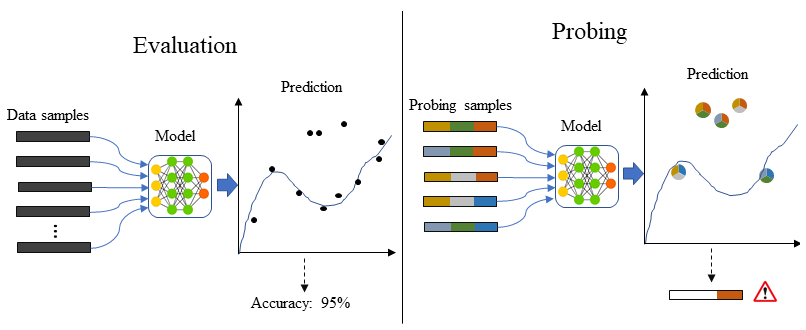
\includegraphics[width=\textwidth]{images_SecureComm/Eva_Prob.png}
\caption{Model evaluation and model probing with controlled data characteristics.}\label{figM:Prob}
\end{figure}

Machine-learning breakthroughs in many fields have been reliant on a precise understanding of data structure and corresponding descriptive labelling to develop more suitable models.
In \textit{automatic speech recognition (ASR)}, tone and emotions can alter the meaning of a sentence significantly. The huge automatically gathered speech datasets however only contain speech snippets and if possible their plain transcripts. While modern speech models are in principle able to learn implicit structures such as emotions without explicit labels, it is impossible to determine the cause for systematic error when they are not. Datasets that contain labelled specialised speech characteristics such as the Ryerson Database of Emotional Speech and Song (RAVDESS) \cite{livingstone2018ryerson} not only allow researchers to identify if their model is susceptible to structural misclassification through targeted probing, but also inspire new methods to capture and understand these implicit structures \cite{haque2019audio}, which in turn leads to design improvements of general speech recognition models \cite{kamper2020multilingual}.



%Prominent network intrusion detection methods as Kitsune \cite{mirsky2018kitsune} or DeepCorr \cite{nasr2018deepcorr} learn structures in the sizes, flags, or interarrival times of packets for decision-making. These \textbf{traffic microstructures} that can be observed when looking sequences of packets or connections reveal information about attack behaviour, but are also influenced by a number of other factors such as network congestion or the transmitted data. However,


In contrast to ASR, no effort has been made so far to monitor or control the effect of similar factors on network traffic to probe these models for specific microstructures, with the current quasi-benchmark NID-datasets pay more attention to the inclusion of specific attacks and topologies rather than the documentation of the generated traffic. This situation has so far led researchers to often simply evaluate a variety of ML-models on these datasets in the hope of edging out competitors, without understanding model flaws and corresponding data structures through targeted probing.


In this chapter, we demonstrate how to produce traffic effectively to probe a state-of-the-art traffic classifier, and why a certain degree of generative \textbf{determinism} is required for this to isolate the influence of traffic microstructures. The model insights and corresponding performance improvements achieved through probing motivate our experimental examination of various influence factors over microstructures and how to control them during traffic generation. 

\textbf{Thesis context:} This chapter builds up on chapter \ref{Chap:Req} by extending the examination of DetGen. Here, we examine DetGen's near-deterministic control over microstructure-shaping factors such as conducted activity, communication failures or network congestion to generate reproducible traffic samples along with corresponding ground-truth labels. %Our motivation stems from the lack of attention that current benchmark datasets spent on these factors.
%how traffic microstructure labelling improves the probing of \textcolor{red}{NIDS} models, and how traffic with controllable microstructures can be generated for this purpose.


% Data containing ground-truth on the traffic generation process to link observable structures with corresponding computational activities is rare, which has so far lead researchers to predominantly apply a number of ML-models to traffic datasets in the hope of edging out competitors. %In-depth analyses regarding which traffic characteristics lead to inaccurate predictions or cause a model to misbehave,
%This overall lack of connection between the nature of intrusion detection data and the applied data-driven detection systems has been identified as a `semantic gap' by Paxson and Sommer \cite{sommer2010outside}, and is seen to be partly responsible for the lack of success machine-learning had in network intrusion detection. This claim has been supported and partly extended by Harang \cite{harang2014bridging} in 2014 and by Liu et al. in 2019 \cite{liu2019machine}.

%By moving from virtual machines to containers, we enable the scalable, modular, and dynamic creation of network traffic datasets. Since containers can be arranged in complex settings with a few commands, it is a lot easier with containers to script a variety of network activities thus increase the heterogeneity and realism of the generated data.

 
%We propose a novel design paradigm that makes generation of network traffic and corresponding attacks significantly more flexible and offers a \textcolor{red}{new level} of insight and reproducibility for traffic microstructures through the use of containerisation. 
The majority of work in this chapter was pubished in ``Examining traffic microstructures to improve model development'' (Henry Clausen and David Aspinall, 2021) and ``Controlling network traffic microstructures for machine-learning model probing'' (Henry Clausen, David Aspinall, and Robert Flood, 2021).


This chapter discusses the following results:

\begin{enumerate}
% an exemplary dataset that is suitable for broad probing of models trained on the CICIDS-17 dataset\cite{sharafaldin2018toward}, as it mirrors its range of protocols and attacks.

\item We demonstrate why model probing with controllable traffic microstructure is a crucial step to understand and ultimately improve model behaviour by probing a state-of-the-art LSTM traffic classifier and lowering its false positives five-fold.

% with this traffic dataset, and demonstrate how to  by understanding where the model fails to process particular traffic structures correctly.

\item We discuss requirements for traffic data suitable to probe models pre-trained on a given NIDS-dataset, and demonstrate how to generate probing traffic effectively through DetGen-IDS, a dedicated probing dataset.

\item We examine experimentally how different factors affect traffic microstructures, and how well they can be controlled in a more effective manner when compared to common VM-based traffic generation setups.

\item We examine how DetGen provides accurate control and labels over traffic microstructures, and experimentally demonstrate the level of provided generative determinism to traditional generation set-ups.
%DetGen, a framework based on a novel design paradigm for generating reproducible small-scale traffic structures with ground-truth labels that contain extensive information about the computational interactions behind it. 

%\item We explain how DetGen enables accurate and \textcolor{red}{quasi-deterministic} control over traffic characteristics as well as corresponding ground truth information, and compare the design advantages to traditional generation set-ups.


%\item We also examine the performance of DetGen \textcolor{red}{in the other direction}, namely the ability to generate traffic with realistic levels heterogeneity, and compare the results against those observed in existing artificially generation NID-datasets.


\end{enumerate}
%
%\begin{itemize}
%
%\item We examine how well DetGen is able to control different types of traffic characteristics, and compare the corresponding \textcolor{red}{determinism} to common VM-based traffic generation setups.
%
%\item We also examine the performance of DetGen \textcolor{red}{in the other direction}, namely the ability to generate traffic with realistic levels heterogeneity, and compare the results against those observed in existing artificially generation NID-datasets.
%
%\item We present an exemplary dataset that is suitable for a broad probing of models trained on the CICIDS-17 dataset, as it mirrors its range of protocols and attacks.
%
%\item We demonstrate the extensive probing of an LSTM-based anomaly detection model with this dataset, and demonstrate how to lower false positives effectively by understanding where the model fails to process particular traffic structures correctly.
%
%\end{itemize}


%DetGen and the DetGen-IDS data are openly accessible for researchers on \textit{GitHub}.


\subsection{Outline}

The remainder of the chapter is organized as follows. Section \ref{SecM:Motivation} discusses the need for generating probing data with sufficient microstructure control before presenting the probing and corresponding improvement of a state-of-the-art intrusion detection model as a motivating example. Section \ref{SecM:ProbData} discusses how to generate probing data appropriately for pretained models, and provides an overview over the DetGen-IDS data.
%provides an overview over the probing dataset that we are releasing and explains why and in what way it mirrors the CICIDS-17 dataset. 
Section \ref{SecM:DetGenMicro} proceeds to examine over which traffic characteristics DetGen exerts control and the corresponding control level.
Section \ref{SecM:Archi} provides details over the design paradigm of DetGen and the resulting advantages over traditional setups, while Section \ref{SecM:Determinism} discusses the level of control DetGen provides when compared to traditional setups. Section \ref{SecM:ProbData} discusses how to generate probing data appropriately for pretained models, and provides an overview over the DetGen-IDS data.
 Section \ref{SecM:Conclusion} concludes our work.
%and \ref{SecM:Refining} we demonstrate how to perform model probing and implement corresponding design improvements on two network intrusion detection models. Section \ref{SecM:Conclusion} concludes the results and discusses limitations of our work and directions for future work.

\subsection{Existing datasets and corresponding ground-truth information}\label{SecM:ExData}

Real-world NID-datasets such as those from the Los Alamos National Laboratory \cite{kent-2015-cyberdata1} (LANL) or the University of Grenada \cite{macia2018ugr} provide large amounts of data from a particular network in the form of flow records. Due to the lack of monitoring and traffic anonymisation, it is impossible for researchers to extract detailed information about the specific computational activity associated with a particular traffic sample.
Synthetic NID-datasets such as the CICIDS-17 and 18 \cite{sharafaldin2018toward} or the UNSW-NB-15 \cite{moustafa2015unsw} aim to provide traffic from a wide range of attacks as well as an enterprise-like topology in the form of \texttt{pcap}-files and flow-statistics. The CICIDS-17 data for example contains 5 days of network traffic from 12 host that include different Windows, Ubuntu, and Web-Server versions, and covers attacks from probing and DoS to smaller SQL-injections and infiltrations.
While some effort is put in the generation of benign activities using activity scripting or traffic generators, we have seen no attention being spent at monitoring these activities accordingly, which leaves researchers with the limited information available through packet inspection. Furthermore, synthetic datasets can be criticised for their limited activity range, such as the CICIDS-17 dataset where more than $95\%$ of FTP-transfers consist downloading the Wikipedia page for ‘Encryption’ \cite{ring2019survey}, which leads to insufficient structural nuances to for effective probing.

%pronounced in commonly used network intrusion datasets such as the CICIDS-17 dataset, where the vast majority of successful FTP-transfers consist of a client downloading a single text file that contains the Wikipedia page for ‘Encryption’.


%DetGen generates traffic with precise control and monitoring over the conducted communication activity as well as various traffic-shaping factors. The scope lies on microscopic traffic-structures that become apparent on a packet- or individual flow-level.

%DetGen separates program executions and traffic capture into distinct containerised environments in order to exclude any background traffic events, and therefore provides precise ground-truth about the computational origin of the traffic, something that is lacking in all network traffic datasets that we are aware of. %By using containerisation, we are furthermore able to control and shield the traffic generation better than in conventional VM-setups, as we demonstrate in Section \ref{SecM:Determinism}, and consequently provide better reproducible data. 
%In order to examine additional effects on traffic microstructures, DetGen simulates influence factors such as network congestion, communication failures, data transfer size, content caching, or application implementation.


\section{Methodology and example}\label{SecM:Motivation}

%\textcolor{red}{Do we need the paragraph below?}



%\subsection{Scope of DetGen}
%\subsection{Improving a classifier with traffic control and microstructure labels}
%\label{SecM:Motivation}


Assume the following problem: You are designing a packet-level traffic classifier which is generating a significant number of false positives, something that is still a common problem for the state-of-the-art \cite{nisioti2018intrusion}. The false positives turn out to be caused by a particular characteristic such as unsuccessful logins or frequent connection restarts. However, existing real-world or synthetic datasets do not contain the necessary information to associate traffic events with these characteristics, which prevents you from identifying the misclassification cause effectively. To address this problem, we need a way to controllably generate and label traffic microstructures caused by these characteristics.
%We designed DetGen to generate traffic with sufficient ground-truth information to allow effective association of such model failures with traffic characteristics.

To provide an example, we look at a \textit{Long-Short-Term Memory} (LSTM) network, a deep learning design for sequential data, by Hwang et al. \cite{hwang2019lstm}, which is designed to classify attacks in web traffic and has achieved some of the highest detection rates of packet-based classifiers in a recent survey \cite{tahaei2020rise}. Through probing we will learn that retransmissions in a packet sequence dramatically deplete the model's classification accuracy. We take the following steps:

\begin{enumerate}
\item [] \textbf{Step 1:} Determine model performance and feed it suitable probing traffic.
\item [] \textbf{Step 2:} Examine the correlation between traffic misclassification scores and the generated traffic microstructure labels to find a likely cause.%, which is strongest for simulated packet reordering.
\item [] \textbf{Step 3:} Examine at which latency levels specific connections are misclassified.

\item [] \textbf{Step 4:} Generate two similar connections, with one exposed to strong packet latency.% to examine how it affects the processing.
\item [] \textbf{Step 5:} Show that by removing retransmission sequences in the pre-processing, misclassification is significantly reduced.
\end{enumerate}

%After training the model on the CICIDS-17 dataset \cite{sharafaldin2018toward}, the biggest source for misclassifications turn out to be packet retransmission sequences. 



%Below, we provide a \textcolor{red}{use-case} to demonstrate how ground-truth information and traffic microstructure control enables effective model probing:

%\section{Use-cases}


%Possible title: \textbf{Exploring the effect of rare events to model performance}
%Our first example looks at how descriptive ground truth information on traffic characteristics can improve a
%In this \textcolor{red}{use-case}, we improve the design of a traffic classification model through the analysis of data separation in dependence of different traffic features. We use a recent traffic classification model by Hwang et al. \cite{hwang2019lstm} as an example, which aims at distinguishing various types of malicious activity from benign traffic. The model achieved some of the highest detection rates of packet-based classifiers in a recent survey \cite{tahaei2020rise} and is claimed to achieve detection and false positive (FP) rates of \textbf{99.7\%} and \textbf{0.03\%} respectively. It classifies connections on a packet-level using a \textit{Long-short-term memory} (LSTM) network \footnote{a deep learning design for sequential data}. 


%This dataset, released by the Canadian Institute for Cyber-security (CIC), contains 5 days of network traffic collected from 12 computers with attacks that were conducted in a laboratory setting. The attack data of this dataset is one of the most diverse among NID datasets and contains SQL-injections, Heartbleed attacks, brute-forcing, various download infiltrations, and cross-site scripting (XSS) attacks.

\textbf{Step 1:} To detect SQL injections, we train the model on the CICIDS-17 dataset \cite{sharafaldin2018toward} (85\% of connections).
%This dataset is the most recent and covers the most attacks of the several existing de-facto benchmark datasets. 
For the evaluation, we also include a set of HTTP-activities generated by DetGen (7.5\%) that mirror the characteristics in the training data, as explained in Section \ref{SecM:ProbData}. %Rather than providing an accurate and realistic detection setting, this example shows how traffic information can be linked to model failures and slumping performance. 
In total, we use 30,000 connections for training and for evaluating the model, or slightly under 2 million packets.
The initially trained model performs relatively well, with an \textit{Area under curve} (AUC)-score %\footnote{a measure describing the overall class separation of the model}
 of \textbf{0.981}, or a detection/false positive rate\footnote{tuned for the geometric mean} of \textbf{96\%} and \textbf{2.7\%}. However, to enable operational deployment the false positive rate would need to be several magnitudes lower \cite{mell2003overview}. 


\begin{figure}
\centering
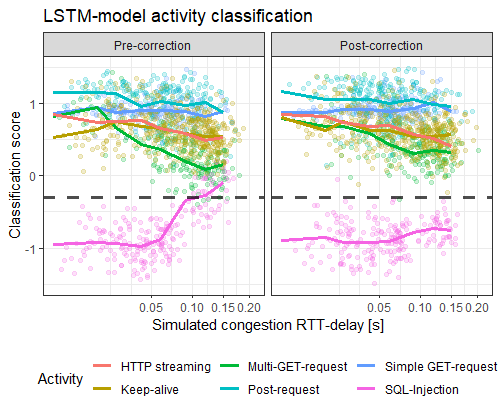
\includegraphics[width=0.99\textwidth]{images_SecureComm/LSTM_classi.png}
\caption{Scores for the LSTM-traffic model before and after the model correction.}\label{figM:LSTM_exp}
\end{figure}


\textbf{Step 2:} Now suppose we want to improve these rates to both detect more SQL-injections and retain a lower false positive rate. To start, we explore which type of connections are misclassified most often. We retrieve the classification scores for all connections and measure their linear correlation to the microstructure labels available for the probing data. The highest misclassification ratio was measured for one of the three SQL injection scenarios (19\% correlation) and connections with multiple GET-requests (11\% correlation). When not distinguishing activities, we measured a high misclassification correlation with simulated packet latency (12\%), which we now examine. More details on this exact procedure can be found in (citation currently blinded).



\textbf{Step 3:} Fig. \ref{figM:LSTM_exp} depicts classification scores of connections in the probing data in dependence of the emulated network latency. The left panel depicts the scores for the initially trained model, while the right panel depicts scores after the model correction that we introduce further down. 
The left panel shows that classification scores are well separated for lower congestion, but increased latency in a connection leads to a narrowing of the classification scores, especially for SQL-injection traffic. Since there are no classification scores that reach far in the opposing area, we conclude that congestion simply makes the model lose predictive certainty. 
Increased latency can both increase variation in observed packet interarrival times (IATs), and lead to packet out-of-order arrivals and corresponding retransmission attempts. Both of these factors can decrease the overall sequential coherence for the model, i.e. that the LSTM-model loses context too quickly either due to increased IAT variation or during retransmission sequences. 


\begin{figure}
\centering
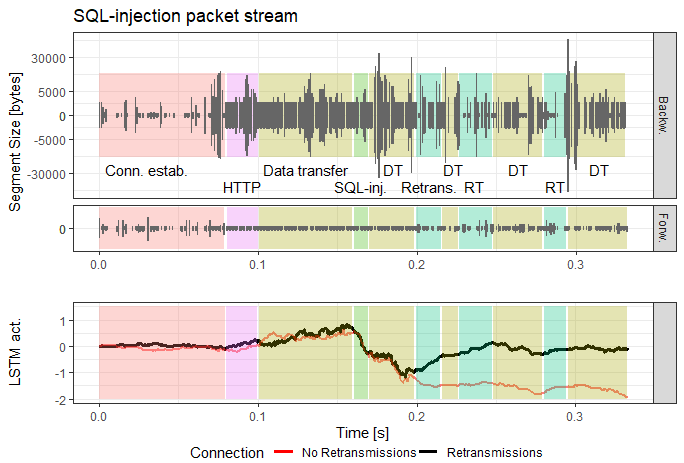
\includegraphics[width=0.99\textwidth]{images_SecureComm/LSTM_activation_new.png}
\caption{LSTM-output activation in dependence of connection phases.}\label{figM:LSTM_act}
\end{figure}

\textbf{Step 4:} We use DetGen to generate two similar connections, where one connection is subject to moderate packet latency and corresponding reordering while the other is not. DetGen's ability to shape traffic in a controlled and deterministic manner allows us to examine the effect of retransmission sequences on the model output and isolate it from other potential influence factors. 
Fig. \ref{figM:LSTM_act} depicts the evolution of the LSTM-output layer activation in dependence of difference connection phases for the connection subject to retransmissions. Depicted are packet segment streams and their respective sizes in the forward and backward direction, with different phases in the connection coloured and labelled. Below is the LSTM-output activation while processing the packet streams. The red line shows the output for the connection without retransmissions\footnote{scaled temporally to the same connection phases} as a comparison.
Initially the model begins to view the connection as benign when processing regular traffic, until the SQL-injection is performed. The model then quickly adjusts and provides a malicious classification after processing the injection phase and the subsequent data transfer, just as it is supposed to. 

The correct output activation is however quickly depleted once the model processes a retransmission phase and is afterwards not able to relate the still ongoing data transfer to the injection phase and return to the correct output activation. When we compare this to the connection without retransmissions, depicted as the red line in Fig. \ref{figM:LSTM_act}, we do not encounter this depletion effect. Instead, the negative activation persists after the injection phase.

\textbf{Step 5:} Based on this analysis, we try to correct the existing model with a simple fix by excluding retransmission sequences at the pre-processing stage. This leads to significantly better classification results during network latency, as visible in the right panel of Fig. \ref{figM:LSTM_exp}. SQL-injection scores are now far-less affected by congestion while scores for benign traffic are also less affected, albeit to a smaller degree.
The overall AUC-score for the model improves to \textbf{0.997} while tuned detection rates improved to \textbf{99.1\%} and false positives to \textbf{0.345\%}, a five-fold improvement from the previous false positive rate of $2.7\%$. 


\section{Refining the notion of benign traffic for anomaly detection}\label{SecM:Refining}

Next, we show how ground-truth traffic information can help produce more coherent clusters and thus refine the benign traffic model in anomaly-detection. In particular, we will examine a 
simplified version of \textit{Kitsune} \cite{mirsky2018kitsune}, a recent deep learning anomaly-detection model based on stacked autoencoders. \textit{Kitsune's} AUC-scores surpassed those of other state-of-the-art methods for a variety of attacks, including various types of Botnet traffic and \textit{man-in-the-middle} attacks.

%for access attacks according to a survey by Nisioti et al. \cite{nisioti2018intrusion}.
The model takes connection packet streams as input, which are pushed through an artificial information bottleneck before reconstruction, which forces the model to learn and compress reoccurring traffic structures. The compressed connection representation is essentially a positional projection into a lower-dimensional vector space, where spatial boundaries around benign traffic can be drawn. For demonstration purposes, we use a widely-used clustering approach for anomaly-detection rather than \textit{Kitsune's} more complex ensemble method. 
%This allows us to project flows into a lower-dimensional vector space, where spatial boundaries around benign traffic can be drawn using clustering to identify anomalous traffic events. The model takes 102 flow summary statistics as input, which include features such as packet size and interarrival statistics, flag occurrencies, or number of flows in window. 
Here, anomalous outliers are detected using the Mahalanobis-distance of a projected connection from identified cluster centers. %The identified clusters therefore serve as structural enclosures of benign behaviour, with the cluster borders acting as separators to abnormal behaviours. 
Benign traffic should ideally be distributed evenly around the cluster centres to allow a tight borders and good separation from actual abnormal behaviour.

Unstructured datasets such as the CAIDA traffic traces assumably contain too much abnormal behaviour to train an anomaly-detection model, which is why we train the model on benign traffic from the CICIDS-17 \cite{sharafaldin2018toward} intrusion detection dataset (80\%). Again, we add 20\% probing traffic consists of HTTP, FTP, SSH, and SMTP communication, using a wide spectrum of settings for examination purposes. Attack data for the evaluation was again provided through the CICIDS-17 dataset, and includes access attacks such as SQL-injections or Brute-Forcing, as well as Mirai botnet traffic. We  train the model with in total 150,000 connections.

\subsection{Projection coherency evaluation}

\begin{table}
\centering
\begin{tabular}{p{1.5cm}|p{3.6cm}|p{3.4cm}|p{3.4cm}}
Label&\textbf{HTTP}&\textbf{File-Sync} & \textbf{Mirai-C\&C}\\ \hline 
\textbf{1}& Get-req. NGINX, low lat.&  Two hosts, low lat. & Command 1, low lat. \vspace{0.1cm} \\ \hline
Results:& \textcolor{myblue}{0.14}\space ,\space\space\textcolor{myred}{0.45} 
&\textcolor{myblue}{0.19}\space ,\space\space\textcolor{myred}{0.27} 
&\textcolor{myblue}{0.03}\space ,\space\space\textcolor{myred}{0.06}\\ \hline \hline
\textbf{2}&Multi-req. NGINX, low lat. & Four hosts, low lat. & Command 2, low lat.\\ \hline
Results:&\textcolor{myblue}{0.32}\space ,\space\space\textcolor{myred}{0.45} 
&\textcolor{myblue}{0.15}\space ,\space\space\textcolor{myred}{0.33} 
&\textcolor{myblue}{0.03}\space ,\space\space\textcolor{myred}{0.04}\\ \hline \hline
\textbf{3}& Post-req. Apache, high lat. &Two hosts, high lat. & Command 3, high lat.\\ \hline
Results:&\textcolor{myblue}{0.17}\space ,\space\space\textcolor{myred}{0.28} 
&\textcolor{myblue}{0.16}\space ,\space\space\textcolor{myred}{0.28} 
&\textcolor{myblue}{0.02}\space ,\space\space\textcolor{myred}{0.04}\\ \hline \hline
\textbf{4}& Multi-req. Apache, high lat. & Four hosts, high lat. & Command 4, high lat.\\ \hline
Results:&\textcolor{myblue}{0.53}\space ,\space\space\textcolor{myred}{2.51} 
&\textcolor{myblue}{0.71}\space ,\space\space\textcolor{myred}{1.31} 
&\textcolor{myblue}{0.03}\space ,\space\space\textcolor{myred}{0.05}\\ \hline \hline
\end{tabular}
\caption{Outline of the traffic settings for examining projection consistency. The numbers below each setting describe the measured Mahalanobis-distances (blue:average, red:maximal) for the corresponding projections.}\label{tabM:Dataset}
\end{table}

Like many approaches that generate representations of benign traffic for anomaly detection, \textit{Kitsune} projects traffic events into a vector-space where traffic clusters and similarities become more apparent. In order for the projection to accurately capture important traffic structures, this projection should be consistent, i.e. traffic events with similar origins and characteristics should be projected to similar positions rather than be dispersed throughout the vector space \cite{hou2017deep}.

%Verifying the projection consistency of a model is not straightforward as usually no or not enough ground-truth information about different traffic characteristics is available to asses if the model is projecting similar traffic to dissimilar positions, or if the traffic just bears some dissimilar characteristics.

To verify the models projection consistency, we generate traffic from near-identical conditions to provide certainty on the expected traffic similarities. We generate a small dataset that consists of HTTP-requests, file-synchronisation, and Botnet communication. For each of the three traffic types we fix four settings that vary in the performed activity and network latency, with the traffic shaping described in Section \ref{SecM:DetGenMicro} being held constant within each setting except for small variations in the transmitted message or file. Table \ref{tabM:Dataset} summarises the traffic for each setting. 

We verify if traffic samples within each group are projected to similar areas by measuring the average and maximum Mahalanobis-distance to quantify the overall dispersion of the samples. The results are displayed in Table \ref{tabM:Dataset} and depicted in Fig. \ref{figM:Subspace_disp}. The first thing to notice is that the model projects samples from each group within the same cluster, thus confirming the capture of a coarse traffic structure. When looking at the traffic dispersion and the corresponding Mahalanobis-distance measurements, we notice that the \textit{multi-request HTTP} traffic as well as the \textit{file-synchronisation} between mutliple computers is much further dispersed than in the other settings, especially when exposed to more latency. We also find that the corresponding dimension, $x_3$, with the most projected dispersion seems to be the same for each of the four settings. This suggests that the cause for the dispersion is the same for the different traffic types. 

We now focus on the influence of input features on the projected positions exclusively in the $x_3$-direction. Here, we can again perform a simple correlation analysis between different the input feature values and the corresponding $x_3$-value. We observe that the arrival time of packet bears the most correlation (5.4\%) for the selected settings. We also see that this influence is concentrated primarily on connections that are opened shortly after a previous connection, with the temporal separation between these two connections apparently being the primary cause for the spread on the $x_3$-axis. The connection interarrival times are naturally an important feature for \textit{Kitsune} to detect attacks such as \textit{Man-in-the-Middle}, which could explain the weight this feature plays in the projection process.

%look at the the influence of the individual flow features on projected position, we notice that even slight differences in the IAT of the preceding and the subsequent flow impacts the projected position quite strongly, which is why only the settings that generate multiple flows are affected.


\begin{figure}
\centering
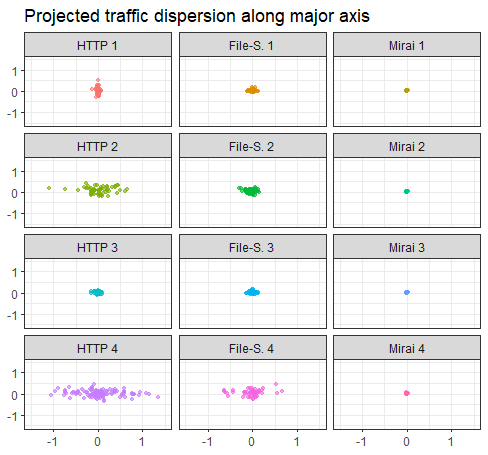
\includegraphics[width=0.5\textwidth]{images_SecureComm/traffic_dispersion.png}
\caption{Dispersion of projected traffic samples from each setting, plotted along the two most dispersed axes.}\label{figM:Subspace_disp}
\end{figure}


%at the effect of sudden connection terminations on an anomaly-detection model by Casas et al. \cite{casas2012unsupervised}. 

\subsection{Investigating individual cluster incoherences}


When examining false-positive and corresponding anomaly scores, we noticed that the model often classifies Brute-Force Web attacks as benign and some HTTP-traffic as anomalous. When examining the projected location of the corresponding connections, we see that most of this HTTP-traffic as well as the Brute-Force attack traffic lie near a particular cluster, depicted in Fig. \ref{figM:Subspace_projection}. A significant portion of traffic in that cluster seems to be spread significantly more across the cluster axis than the rest of the traffic in that cluster, leading to an inflated radius that partially encompasses Brute-Force traffic. 

When cross-examining the traffic in this cluster with the probing data, we see that HTTP-traffic with the label "Sudden termination" are distributed across the cluster axis in a similar fashion, also depicted in Fig. \ref{figM:Subspace_projection}, suggesting the conclusion that this type of traffic causes the inflated cluster radius. DetGen generates traffic with the label "Sudden termination" as half-open connections which were dropped by the server due to network failure. One defining characteristic of such connections are that they are not closed with a termination handshake using FIN-flags. To better capture this defining characteristics in the modelling process, we included an additional feature attached to the end of a packet sequence that indicates a proper termination with FIN-flags in the modelling process.
The newly trained model now projects "Sudden termination" connections into a different cluster, which leads to a far better cluster coherence. The detection rate on Brute-Force attack traffic could thus be improved from \textbf{89.7\%} to \textbf{94.1\%}.

\begin{figure}
\centering
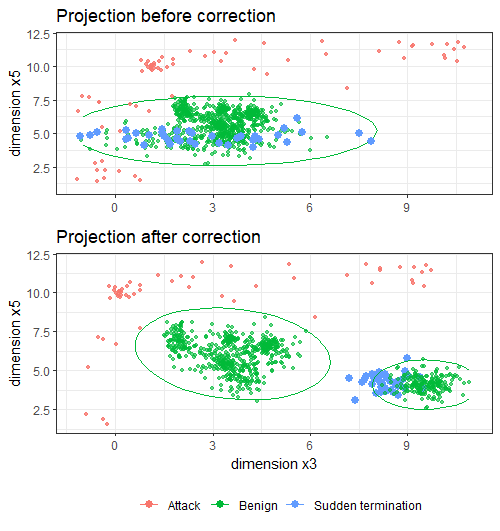
\includegraphics[width=0.5\textwidth]{images_SecureComm/Subspace_projection_new3.png}
\caption{Scores for the LSTM-traffic classification model in dependence of simulated network congestion, along with the classification threshold}\label{figM:Subspace_projection}
\end{figure}





%\textcolor{red}{To be added}

%\section{Examining traffic microstructures}



\section{Traffic microstructures and their influence factors}\label{SecM:DetGenMicro}

%\textcolor{red}{...ALP microstructure}
The biggest and most obvious influence on traffic microstructures is the choice of the application layer protocols. For this reason, the range of protocols is often used as a measure for the diversity of a dataset. However, while the attention to microstructures in current NID-datasets stops here, computer communication involves a myriad of other different computational aspects that shape observable traffic microstructures. Here, we highlight and quantify the most dominant ones, which will act as a justification for the design choices we outline in Section \ref{SecM:ExtInfls}. We look at both findings from previous work as well as our own experimental results.
%Protocols such as HTTP/TLS perform vastly different tasks than protocols such as Peer-2-Peer or SMB, and thus perform different handshakes, experience different waiting times, transfer data in different intervals, or trigger different additional connections. However, 

%In order to enable sufficient and reproducible control over the generated traffic and provide the corresponding descriptive ground truth information, we first must understand what factors shape the traffic generation process. 
%Computer communication involves a myriad of different computational aspects, and no research so far has been conducted to quantify how much influence each of them has on traffic structures. We highlight and quantify the influence of the most important influence factors on the traffic microstructures observed on individual devices. These will act as a justification for the design choices we outline in Section \textcolor{red}{...}.

%\paragraph{1. Application layer protocols} 
%Without doubt the biggest impact on the captured traffic microstructures is the choice or combination of the application layer protocols. Protocols such as HTTP/TLS perform vastly different tasks than protocols such as Peer-2-Peer or SMB, and thus perform different handshakes, experience different waiting times, transfer data in different intervals, or trigger different additional connections. 

%\begin{figure}
%\centering
%\begin{subfigure}[b]{0.46\textwidth}
%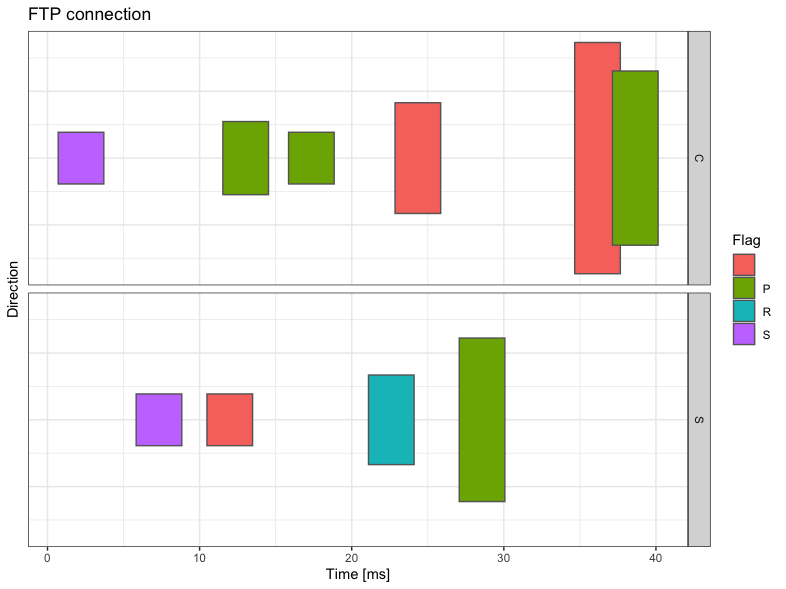
\includegraphics[width=\textwidth]{images_SecureComm/FTP.png}
%\caption{Packet sequence in FTP connection}
%\end{subfigure}
%~
%\begin{subfigure}[b]{0.46\textwidth}
%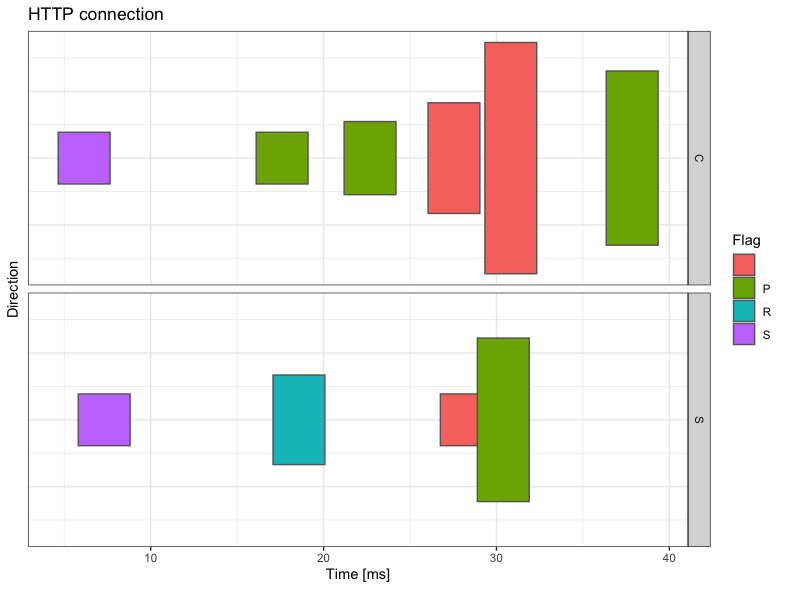
\includegraphics[width=\textwidth]{images_SecureComm/HTTP.png}
%\caption{Packet sequence in HTTP connection}
%\end{subfigure}
%\end{figure}
 
\paragraph{1. Performed task and application.}
The conducted computational task as well as the corresponding application ultimately drives the communication between computers, and thus hugely influences characteristics such as the direction of data transfer, the duration and packet rate, as well as the number of connections established. These features are correspondingly used extensively in application fingerprinting, such as by Yen et al. \cite{yen2009browser} or Stober et al. \cite{stober2013you}. %Fig. \ref{figM:Browser} provides as an example the packet-per-connection differences between different browser choices.

%\begin{figure}
%\centering
%\begin{subfigure}[t]{0.38\textwidth}
%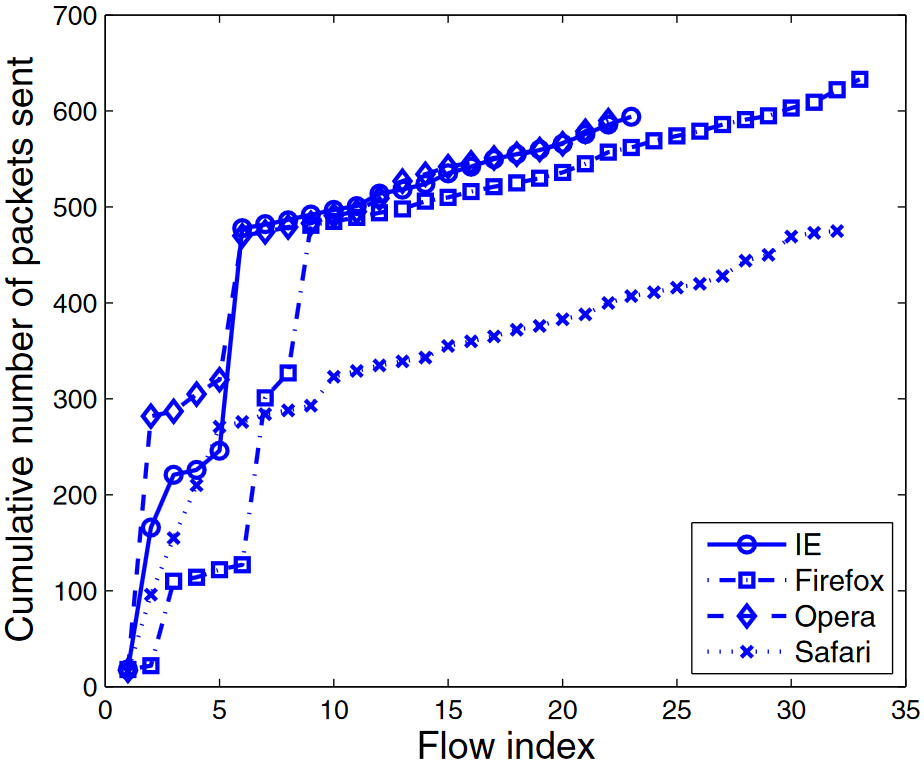
\includegraphics[width=\textwidth]{images_SecureComm/Browser.png}
%\caption{Number of packets sent from a browser, accumulated over all flows that comprise the retrieval. Taken from \cite{yen2009browser}.}\label{figM:Browser}
%\end{subfigure}
%%~
%\begin{subfigure}[t]{0.58\textwidth}
%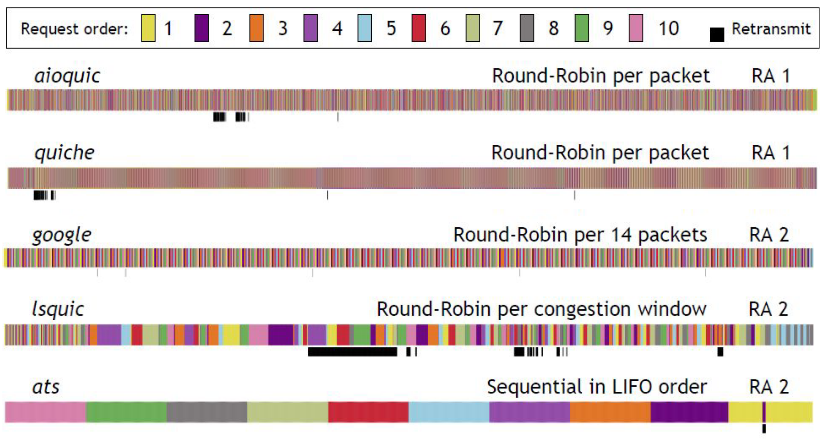
\includegraphics[width=\textwidth]{images_SecureComm/Protocol_differences.png}
%\caption{Comparison of QUIC connection request multiplexing for selected implementations, taken from \cite{marx2020same}.}\label{figM:QUIC}
%\end{subfigure}
%\end{figure}


\paragraph{2. Application layer implementations.}
Different implementations for TLS, HTTP, etc. can yield different computational performance and can perform handshakes differently and differ in multiplexing channel prioritisation, which can significantly impact IAT times and the overall duration of the transfer, as shown in a study by Marx et al. \cite{marx2020same} for the QUIC/HTTP3 protocol\footnote{Fig. 2 in \cite{marx2020same} illustrates these differences in a nice way}. 
%Fig. \ref{figM:QUIC} depicts differences in channel prioritisation for different QUIC-implementations.


\paragraph{3. LAN and WAN congestion.}
Low available bandwidth, long RTTs, or packet loss can have a significant effect on TCP congestion control mechanisms that influence frame-sizes, IATs, window sizes, and the overall temporal characteristic of the sequence, which in turn can influence detection performance significantly as shown in Section \ref{SecM:Motivation}.


\begin{figure}
\centering
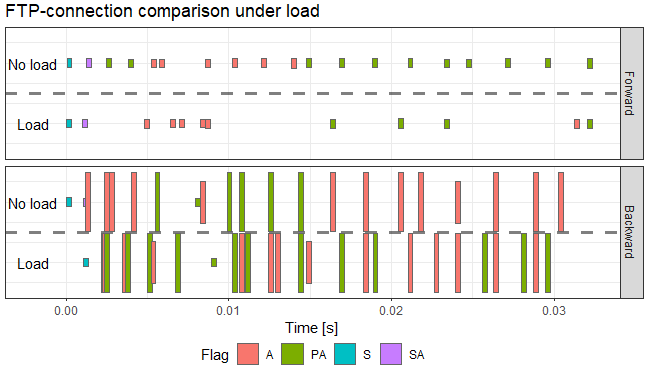
\includegraphics[width=0.9\textwidth]{images_SecureComm/FTP_load.png}
\caption{Packet-sequence similarity comparison under different load.} % Note that under load, the host sends significantly less packets.}
\label{figM:FTP_load}
\end{figure}

\paragraph{4. Host level load.}
In a similar manner, other applications exhibiting significant computational load (CPU, memory, I/O) on the host machine can affect the processing speed of incoming and outgoing traffic, which can again alter IATs and the overall duration of a connection. An example of this is visible in Fig. \ref{figM:FTP_load}, where a FTP-client sends significantly fewer \texttt{PUSH}-packets when under heavy computational load. Colours indicate packet flags while the height of the packets indicates their size. This effect is dependent on the application layer protocol, where at a load number of $3.5$ we see about $60\%$ less upstream data-packets while the downstream is only reduced by $10\%$, compared to HTTP where both downstream and upstream packet rates are throttled by about $40\%$.

%\textcolor{red}{expand this}




\paragraph{5. Caching/Repetition effects.}
Tools like cookies, website caching, DNS caching, known hosts in SSH, etc. remove one or more information retrieval requests from the communication, which can lead to altered packet sequences and less connections being established. For caching, this can result in less than $10\%$ of packets being transferred, as shown by Fricker et al. \cite{fricker2012impact}. 

% parts of a communication being skipped and lead to differences in the captured traffic between initial and subsequent connections.

%\begin{table}[h!]
%\centering
%\begin{tabular}{l|l|l|>{\bfseries}l}
%Time& Source-IP &Destination-IP& Dest. Port\\ \hline
%13:45:56.8 & 192.168.10.9 & 192.168.10.50 &    21 \\ \hline
%13:45:56.9 & 192.168.10.9 & 192.168.10.50 &  10602\\ \hline
%13:45:57.5 & 192.168.10.9 & 69.168.97.166 &   443\\ \hline
%13:45:59.1 & 192.168.10.9 &  192.168.10.3 &    53\\ \hline
%13:46:00.1 & 192.168.10.9 & 205.174.165.73 &   8080\\ \hline
%\end{tabular}
%\caption{Exemplary activity interval for host 192.168.10.9 in the CICIDS-17 dataset, containing FTP-, HTTPS- and DNS-, as well as additional unknown activity.}\label{tabM:Sess}
%\end{table}

%\paragraph{4. Captured traffic from background activity} 
%In traditional setups, all traffic generated on a host is recorded in the same capture, which makes it hard if not impossible to disentangle traffic from different activities and match them to their origin. Capturing background traffic typically leads to additional flows within the given time interval. $74\%$ of SSH-connections and more than $95\%$ of FTP- and HTTPS-connections in the CICIDS-17 dataset lie within a 5-second interval of connections from other background activity on the same network interface, as depicted in Table \ref{tabM:Sess}.



%\begin{figure}
%\centering
%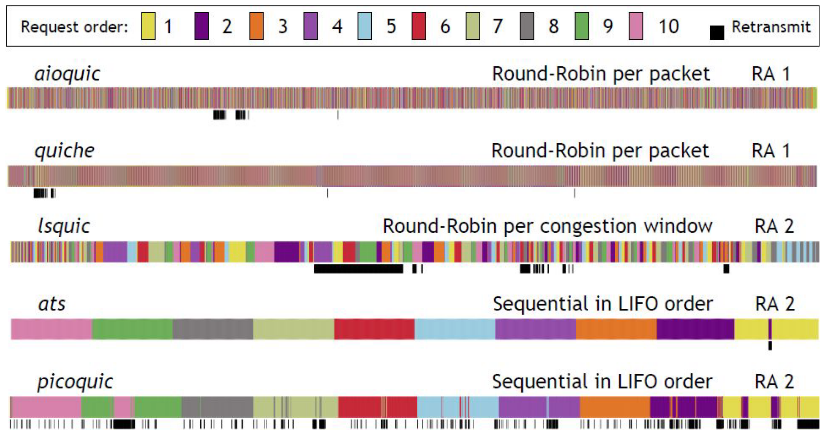
\includegraphics[width=0.65\textwidth]{images_SecureComm/Proto_differences_small.png}
%\caption{Comparison of QUIC connection request multiplexing for selected implementations, taken from \cite{marx2020same}.}
%\end{figure}



%\paragraph{6. Transferred data} 
%The amount of transferred data influences the overall packet numbers. Furthermore, the content of the data can potentially impact packet rates and sizes, such as shown by Biernacki \cite{biernacki2017analysis} for streaming services.

\paragraph{6. User and background activities.}
The choice and usage frequency of an application and task by a user, sometimes called \textit{Pattern-of-Life}, governs the larger-scale temporal characteristic of a traffic capture, but also influences the rate and type of connections observed in a particular time-window \cite{aparicio2017using}. The mixing of different activities in a particular time-window can severely impact detection results of recent sequential connection-models, such as by Radford et al. \cite{radford2018network} or by Clausen et al. \cite{henryLSTM}. To quantify this effect, we look at FTP-traffic in the CICIDS-17 dataset. As explained in Section \ref{SecM:ExData}, the FTP-traffic overwhelmingly corresponds to the exact same isolated task, and should therefore spawn the same number of connections in a particular time window. However, we observe additional connections from other activities within a 5-second window for $68\%$ of all FTP-connections, such as depicted in Table \ref{tabM:Sess}, which contains FTP-, HTTPS- and DNS-, as well as additional unknown activity.
%Since we are focusing on traffic microstructures, we currently omit this impact factor from our analysis. 

\begin{table}[h!]
\centering
\begin{tabular}{l|l|l|>{\bfseries}l}
Time& Source-IP &Destination-IP& Dest. Port\\ \hline
13:45:56.8 & 192.168.10.9 & 192.168.10.50 &    21 \\ \hline
13:45:56.9 & 192.168.10.9 & 192.168.10.50 &  10602\\ \hline
13:45:57.5 & 192.168.10.9 & 69.168.97.166 &   443\\ \hline
13:45:59.1 & 192.168.10.9 &  192.168.10.3 &    53\\ \hline
13:46:00.1 & 192.168.10.9 & 205.174.165.73 &   8080\\ \hline
\end{tabular}
\vspace{0.2cm}
\caption{5-second window for host 192.168.10.9 in the CICIDS-17 dataset.}\label{tabM:Sess}
%\vspace{-1cm}
\end{table}


Other prominent factors that we found had less effect on traffic microstructures include:

\paragraph{7. Networking stack load.}
TCP or IP queue filling of the kernel networking stack can increase packet waiting times and therefore IATs of the traffic trace, as shown by \cite{sequeira2013influence}. In practice, this effect seems to be constrained to large WAN-servers and routers. When varying the stack load in otherwise constant settings on an Ubuntu-host, we did not find any notable effect on packet sequences when comparing the corresponding traffic with a set of three similarity metrics. More details on this setting and the metrics can be found in Section \ref{SecM:Determinism}.

% and we did not find any effect on packet-sequences for various amounts of load generated with iPerf for a regular UNIX host.


%\paragraph{TCP congestion management implementation}
%Different versions of the TCP congestion manager exist on Windows and Linux such as TCP Reno/Tahoe, which can have minor influence on the traffic, as shown by Grieco et al. \cite{grieco2004performance}. 
%Existing implementations on a machine stay mostly constant, which is why we also omit this variable at the moment.
% Implementations within a machine should stay constant.

\paragraph{8. Network configurations.}
Network settings such as the MTU or the enabling of TCP Segment Reassembly Offloading have effects on the captured packet sizes, and have been exploited in IP fragmentation attacks. However, these settings have been standardised for most networks, as documented in the CAIDA traffic traces \cite{walsworth2015caida}.

%\subsection{Generative determinism of DetGen}



\vspace{0.3cm}
We designed DetGen to control and monitor factors 1-6 to let researchers explore their impact on their traffic models, while omitting factors 7 and 8 for the stated reasons.

\section{DetGen: precisely controlled data generation}\label{SecM:Archi}

%DetGen is a container-based network traffic that we developed to enable repeatable, realistic, and flexible network experiments. DetGen is built on top of the widely used Mininet testbed \textcolor{red}{insert citation} and implements controllable communication scenarios for benign and attack traffic generation.

%\section{Background}\label{SecM:b8ackground}



\subsection{Design overview}

Detgen is a container-based network traffic generation framework that distinguishes itself by providing precise control over various traffic characteristics and providing extensive ground-truth information about the traffic origin. % that we developed to enable repeatable, controllable, and \textcolor{red}{informative} network experiments. 
In contrast to the pool of programs running in a VM-setup, such as used in the generation of the CICIDS-17 and 18 \cite{sharafaldin2018toward}, or UGR-16 \cite{macia2018ugr}, DetGen separates program executions and traffic capture into distinct containerised environments in order to shield the generated traffic from external influences.% and enable the fine-grained control of traffic shaping factors.
Traffic is generated from a set of scripted \textit{scenarios} that define the involved devices and applications and strictly control corresponding influence factors. 
Fig. \ref{figM:Setup_comp} provides a comparison of the DetGen-setup and traditional VM-based setups and highlights how control and monitoring is exerted.
%offer the researcher to modify and label the conducted activity from a variety of \textcolor{red}{angles} and randomisations. %Containers communicate in a virtual network created with Mininet along with virtual software switches, Ethernet links, routers, and firewalls. %The network is then populated with containers ,which perform a variety of activities for traffic generation. The conducted activities are composed of scripted \textit{scenarios} (\textcolor{red}{give examples here}), but subject to a high degree of randomisation. The captured traffic events are labelled individually after the specific generating action.

\begin{figure}
\centering
\begin{subfigure}[b]{0.48\textwidth}
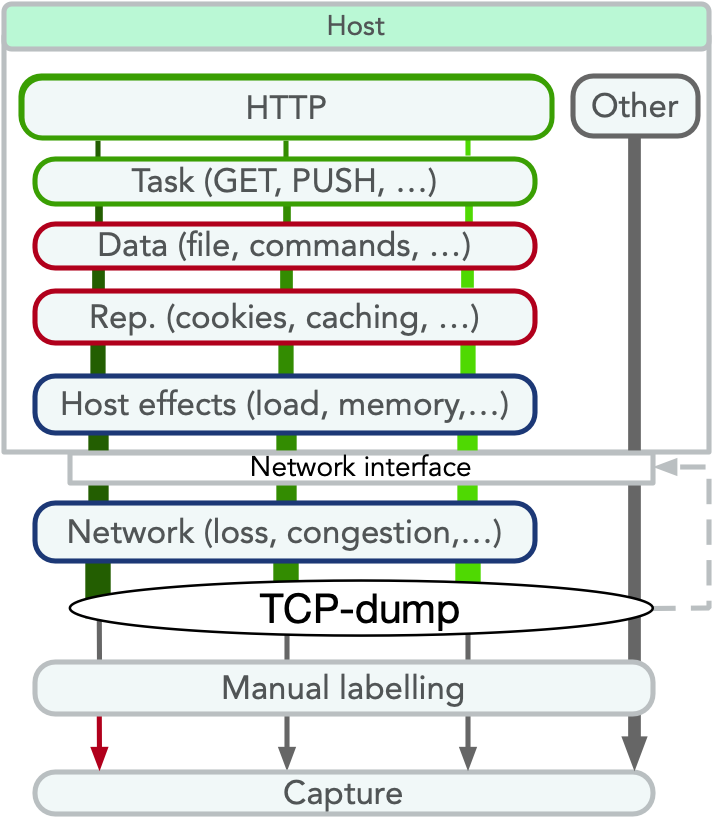
\includegraphics[width=\textwidth]{images_SecureComm/VM_setup_final.png}
\vspace{0.0cm}
\vspace{-0.09cm}
%\caption{Traditional capture setup}
\end{subfigure}
%~
\begin{subfigure}[b]{0.48\textwidth}
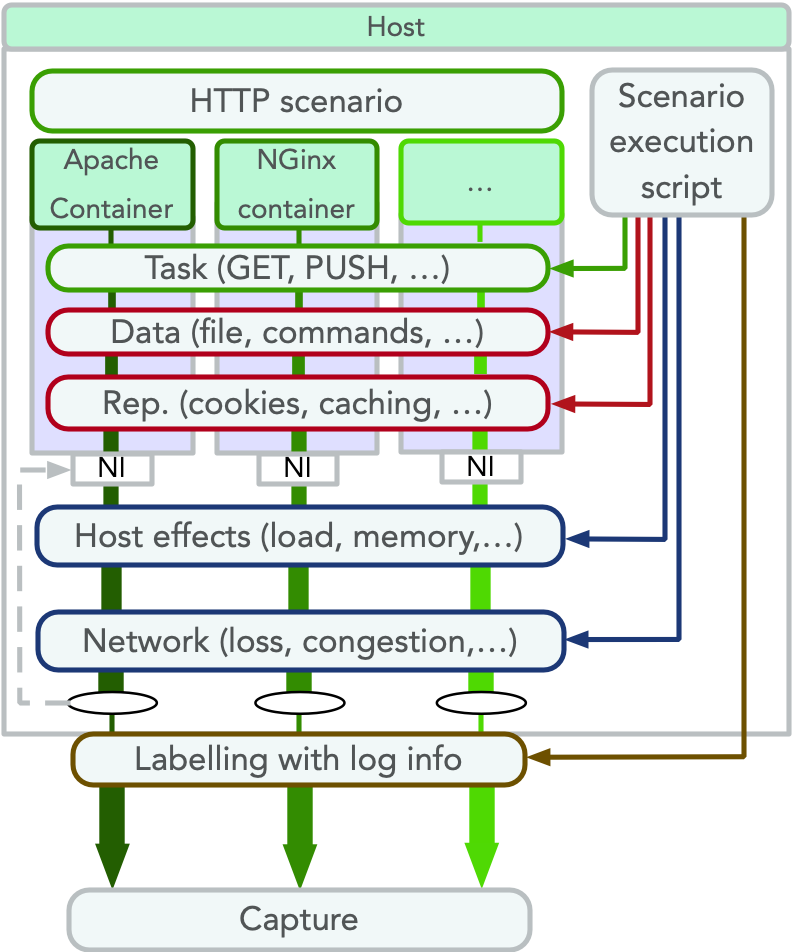
\includegraphics[width=\textwidth]{images_SecureComm/Docker_setup_final.png}
\vspace{0.0cm}
\vspace{-0.4cm}
%\caption{DetGen container setup}
\end{subfigure}
\caption{Traditional traffic-generation-setups (left), and DetGen (right).}\label{figM:Setup_comp}
\end{figure}

\subsection{Containerisation and activity isolation}
%\textcolor{red}{to do:need to improve}
%Containers are standalone packages that contain an application along with all necessary dependencies using OS-level virtualisation. In contrast with standard Virtual machines (VMs), containers forego a hypervisor and the shared resources are instead kernel artifacts that can be shared simultaneously across several containers, leading to minimal CPU, memory, and networking overhead \cite{kolyshkin2006virtualization}.

%\textcolor{red}{Although this prevents the host environment from running different operating systems, containerisation incurs minimal CPU, memory, and networking overhead whilst maintaining a great deal of isolation} \cite{kolyshkin2006virtualization}. 
As we will demonstrate in Section \ref{SecM:Determinism}, containers provide significantly more isolation of programs from external effects than regular OS-level execution. This isolation enables us to monitor processes better and create more accurate links between traffic events and individual activities than on a virtual machine were multiple processes run in parallel and generate traffic. The corresponding one-to-one correlation between processes and network traces allows us to capture traffic directly from the process and produce labelled datasets with granular ground truth information.

Additionally, containers are specified in an image-layer, which is unaffected during the container execution. This allows containers to be run repeatedly whilst always starting from an identical state, allowing a certain level of \textbf{determinism} and reproducibility in the data generation.%In combination with the container isolation, this allows us to perform network experiments that can be easily reproduced by anyone on any platform \textcolor{red}{insert citation}. 

%The container network interface provides the connection between a network namespace and the container runtimes. We want to \textcolor{red}{highlight} that multiple containers can share on network interface, which enables us to generate traffic from multiple applications over one network address in order to emulate \textcolor{red}{fully functional network hosts}.
 

%\subsection{Activity generation}\label{SecM:Scenarios}
%
%\subsubsection*{Scenario.}
%We define a \emph{scenario} as a composition of containers conducting a specific interaction. Each scenario produces traffic from a setting with two (client/server) or more containers, with traffic being captured from each container's perspective. This constructs network datasets with total interaction capture, as described by Shiravi et al. \cite{shiravi2012toward}.
%Examples may include an FTP interaction, an online login form paired with an SQL database, or a C\&C server communicating with an open backdoor. %A full list of currently implemented scenarios can be found in Section \textcolor{red}{\ref{SecM:ExistScen}}.
%%Each scenario is designed to be easily started via a single script and can be repeated indefinitely without further instructions, therefore allowing the generation of large amounts of data.
%Our framework is modular, so that individual scenarios are configured, stored, and launched independently. %Adding or reconfiguring a scenario has no effect on the remaining framework.
%We provide a complete list of implemented scenarios in Table \ref{tabM:scen} in the Appendix.
%%When composing different settings, we most emphasised the inclusion of different \textbf{application layer protocols} such as HTTP or SSH, followed by the inclusion of different corresponding \textbf{applications} such as NGINX or Apache that steer the communication. We are currently aiming to also include options to use different \textbf{application layer implementations} such as TLS1.3 vs TLS1.2.
%
%\subsubsection*{Task.} \label{SecM:Subscenarios}
%
%To provide a finer grain of control over the traffic to be generated, we create a catalogue of different tasks that allow the user to specify the manner in which a scenario should develop. %The aim of having multiple tasks for each scenario is to explore the full breadth of a protocol or application's possible traffic behaviour. For instance, the SSH protocol can be used to access the servers console, to retrieve or send files, or for port forwarding, all of which may or may not be successful. It is therefore appropriate to script a number of tasks that cover this range of tasks.
%%To implement tasks, we first examine the functionality of the underlying protocol and scenario setting before proceeding to adding tasks to the catalogue. 
%To explore the breadth of the corresponding traffic structures efficiently, we prioritise tasks that cover aspects such as the direction of file transfers (e.g. GET vs POST for HTTP), the amount of data transferred (e.g. HEAD/DELETE vs GET/PUT), or the duration of the interaction (e.g. persistent vs non-persistent tasks) as much as possible. For each task, we furthermore add different failure options for the interaction to not be successful (e.g. wrong password or file directory). 

%Subscenarios are specific to particular scenarios and can be specified when launching that scenario.

%The same applies to malicious activity. For instance, it would be naive for an SSH password bruteforcing scenario to always successfully guess a user's password. Instead, we include a second subscenario in which the password bruteforcer fails.

%\subsubsection*{Input randomisation}\label{SecM:randomsubscen}

%Scripting activities that are otherwise conducted by human operators often leads to a loss of random variation that is normally inherent to the activity.
%\textcolor{red}{As mentioned in Section \ref{SecM:problems}, the majority of successful FTP transfers in the CIC-IDS 2017 data consist of a client downloading a single text file.} In reality, file sizes, log-in credentials, and many other variables included in an activity are more or less drawn randomly, which naturally influences traffic quantities such as packet sizes or numbers.

%We identify variable input parameters within scenarios and corresponding tasks and systematically draw them randomly from suitable distributions. Passwords and usernames, for instance, are generated as a random sequence of letters with a length drawn from a truncated Cauchy distribution, before they are passed to the corresponding container. Files to be transmitted are selected at random from a larger set of files, covering different sizes and file names.

%\begin{figure}
%\centering 
%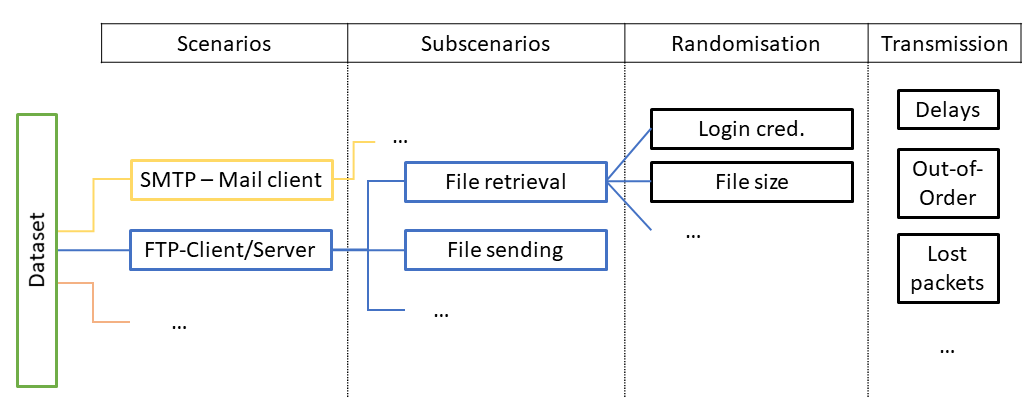
\includegraphics[width=0.5\textwidth]{images_SecureComm/scenario_branching.PNG}
%\caption{Visualisation of the different levels at which traffic variation is introduced in DetGen.}
%\label{figM:branching}
%\end{figure}



\subsection{Simulation of external influence}\label{SecM:ExtInfls}

\subsubsection*{Caching/Cookies/Known server.}

Since we always launch containers from the same state, we prevent traffic impact from \textbf{repetition effects} such as caching or known hosts. If an application provides caching possibilities, we implement this as an option to be specified before the traffic generation process.


\subsubsection*{Network effects.}

%Docker communication takes place over virtual bridge networks, 

%Communication between containers takes place over a virtual bridge network, which provides far higher and more reliable throughput than in real-world networks. Gates and Warshavsky \cite{iperf} measured a bandwidth of over 90 Gbits/s without any lost packets using iPerf.8 This allows us to guarantee reliable and reproducible communication and thus remove external network effects on the captured traffic.


Communication between containers takes place over a virtual bridge network, which provides far higher and more reliable throughput than in real-world networks \cite{iperf}. To retard and control the network reliability and congestion to a realistic level, we rely on \emph{NetEm}, an enhancement of the Linux traffic control facilities for emulating properties of wide area networks from a selected network interface \cite{hemminger2005network}.

%Virtual bridge networks furthermore enable us to retard and control the network reliability and congestion to a realistic level by using emulation tools. NetEm is an enhancement of the Linux traffic control facilities for emulating properties of wide area networks such as high latency, low bandwidth or packet corruption by adding delay, packet loss, duplication etc. to packets outgoing from a selected network interface \cite{hemminger2005network}.

We apply NetEm to the network interface of a given container, providing us with the flexibility to set each container's network settings uniquely. In particular, packet delays are drawn from a Paretonormal-distribution while packet loss and corruption are drawn from a binomial distribution, which has been found to emulate real-world settings well \cite{jurgelionis2011empirical}. Distribution parameters such as mean or correlation as well as available bandwidth can either be manually specified or drawn randomly before the traffic generation process.

%To retard the quality of the Docker network to realistic levels, we rely on emulation tools. As discussed in section \ref{SecM:network}, Netem is a Linux command line tool that allows users to artificially simulate network conditions such as high latency, low bandwidth or packet corruption in a flexible manner.

%Although it is relatively straightforward to apply Netem commands to a Docker Bridge network, we decided not to invoke Netem in this manner as this would cause all network settings of all containers to be identical, such as all containers in a scenario having a latency of 50ms. Instead, we developed a wrapping script that applies Netem commands to the network interface of a given container, providing us with the flexibility to set each container's network settings uniquely. This script randomizes the values of each parameter, such as packet drop rate, bandwidth limit, latency, ensuring that every run of a scenario has some degree of network randomisation if desired.

\subsubsection{Host load.}

We simulate excessive computational load on the host with the tool \emph{stress-ng}, a Linux workload generator. Currently, we only stress the CPU of the host, which is controlled by the number of workers spawned. Future work will also include stressing the memory of a system. We have investigated how stress on the network sockets affects the traffic we capture without any visible effect, which is why we omit this variable here. 

%\subsection{Data generation}
%
%\subsubsection*{Execution script.}
%
%DetGen generates traffic through executing execution script that are specific to the scenario. The script creates the virtual network and populates it with the corresponding containers. The container network interfaces of the containers are then subjected to the NetEm chosen settings and the host is assigned the respective load before the inputs for the chosen task are prepared and mounted to the containers. 
%
%%The user can then choose how long and how often to execute the scenario. Once the activity is terminated, the script takes down the network and containers, and repeats the process for the next repetition. Randomised settings are drawn anew for each repetition.

%\subsubsection*{Labelling and traffic separation.}
%
%Each container network interface is hooked to a \emph{tcpdump}-container that records the packets that arrive or leave on this interface. Combined with the described process isolation, this setting allows us to exclusively capture traffic that corresponds to the conducted activity and exclude any background events. The execution script then stores all parameters (conducted task, mean packet delay, ...) and descriptive values (input file size, communication failure, ...) for the chosen settings.

%\subsection{Network creation and population}

%To enable communication between containers, we build our framework on top Mininet \textcolor{red}{insert citation} to create virtual networks with customisable topology. 
%\textcolor{red}{A topology can be passed to a topology-creation wrapper in matrix form, with diagonal values representing the type of device (switch, container, router, ...), and off-diagonal indicating links}. This allows the import of larger, automatically generated topologies from tools such as \textcolor{red}{insert citation}. 

%\textcolor{red}{maybe something about subnets}. 


\section{Traffic control and generative determinism of DetGen}\label{SecM:Determinism}
We now assess the claim that DetGen controls the outlined traffic influence factors sufficiently, and how similar traffic generated with the same settings looks like. We also demonstrate that this level of control is not achievable on regular VM-based NIDS-traffic-generation setup.

To do so, we generate traffic from three traffic types, namely HTTP, file-synchronisation, and botnet-C\&C, each in four configurations that varied in terms of conducted activity, data/credentials as well as the applied load and congestion. Within each configuration all controllable factors are held constant to test the experimental determinism and reproducibility of DetGen's generative abilities. 
As a comparison, we use a regular VM-based setup, were applications are hosted directly on two VMs that communicate over a virtual network bridge that is subject to the same NetEm effects as DetGen, such as depicted in Fig. \ref{figM:Setup_comp}. Such a setup is for example used in the generation of the UGR-16 data \cite{macia2018ugr}.


To measure how similar two traffic samples are, we devise a set of similarity metrics that measure dissimilarity of overall connection characteristics, connection sequence characteristics, and packet sequence characteristics:


\begin{figure}
\centering
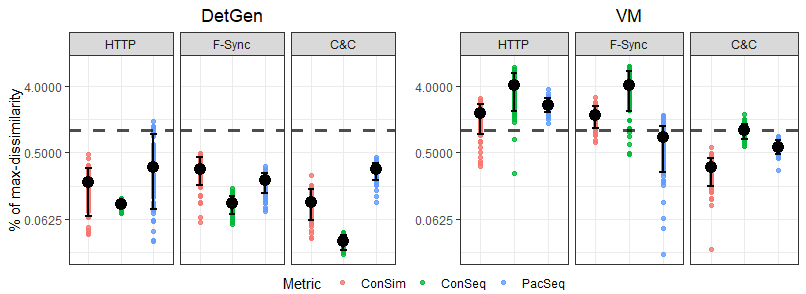
\includegraphics[width=0.99\textwidth]{images_SecureComm/Exp111.png}
\caption{Dissimilarity scores for DetGen and a regular VM-setup, on a log-scale.}\label{figM:determ-metric}
\end{figure}

\begin{itemize}
\item \textbf{Overall connection similarity} We use the 82 flow summary statistics (IAT and packet size, TCP window sizes, flag occurrences, burst and idle periods) provided by CICFlowMeter \cite{lashkari2017characterization}, and measure the cosine similarity between connections, which is also used in general traffic classification \cite{aun2017review}.
\item \textbf{Connection sequence similarity} 
To quantify the similarity of a sequence of connections in a retrieval window, we use the following features to describe the window, as used by Yen et al. \cite{yen2009browser} for application classification: The number of connections, average and max/min flow duration and size, number of distinct IP and ports addresses contacted. We then again measure the cosine similarity based on these features between different windows. 
\item \textbf{Packet sequence similarity} To quantify the similarity of packet sequences in handshakes etc., we use a Markovian probability matrix for packet flags, IATs, sizes, and direction conditional on the previous packet. We do this for sequences of 15 packets and use the average sequence likelihood as this accommodates better for marginal shifts in the sequence. %If connections are completely similar, the conditional probabilities and thus the likelihoods should converge to one.
\end{itemize}

We normalise all dissimilarity scores by dividing them by the maximum dissimilarity score measured for each traffic type to put the scores into context.
For each configuration, we generate 100 traffic samples and apply the described dissimilarity measures to 100 randomly drawn sample pairs. Fig. \ref{figM:determ-metric} depicts the resulting dissimilarity scores on a log-scale.
%, while Table \ref{tabM:Dataset} describes the different settings and the corresponding average dissimilarity scores.

\begin{figure}
\centering
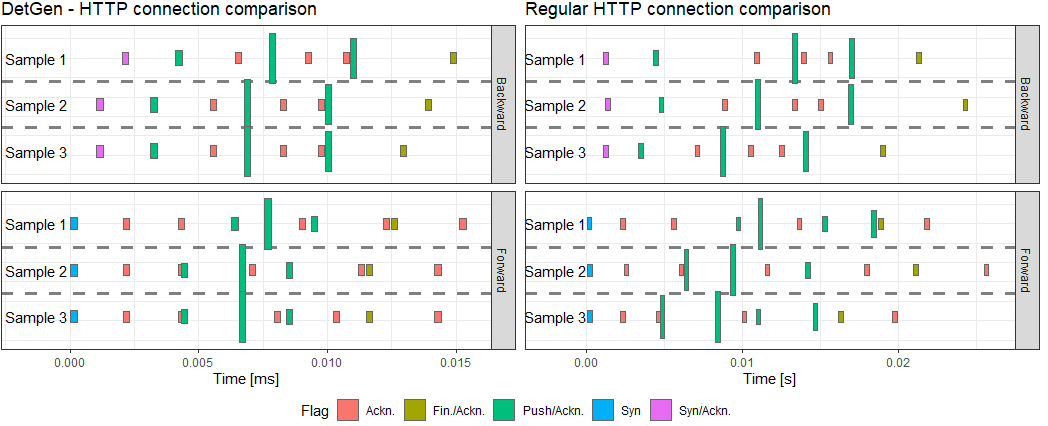
\includegraphics[width=0.99\textwidth]{images_SecureComm/Detgen_Reg_HTTP_comp_crop.png}
\caption{Packet-sequence similarity comparison for HTTP-activity for DetGen and a regular setting.}\label{figM:HTTP-seq}
\end{figure}

The DetGen-scores yield consistently less than $1\%$ of the dissimilarity observed on average for each activity. Scores are especially low when compared to traffic groups collected in the VM setting, which are consistently more dissimilar, in particular for connection-sequence metrics, where the average dissimilarity is more than 30 times higher than for the DetGen setting. Manual inspection of the VM-capture showed that high dissimilarity is caused by additional flow events from background activity (OS and application HTTP, NTP, DNS, device discovery) being present in about $24\%$ of all captures.
. While sequential dissimilarity is roughly the same for the DetGen- and the VM-settings, overall connection similarity for the VM-setting sees significantly more spread in the dissimilarity scores when computational load is introduced.

Fig. \ref{figM:HTTP-seq} depicts an exemplary comparison between HTTP-samples generated using DetGen versus generation using the VM-setup. Colours indicate packet flags while the height of the packets indicates their size. Even though samples from DetGen are not perfectly similar, packets from the VM-setup are subject to more timing perturbations and reordering as well as containing additional packets. Additionally, the packet sizes vary more in the regular setting.

These results confirm that DetGen exerts a high level of control over traffic shaping factors while providing sufficient determinism to guarantee ground-truth traffic information.

\section{Reconstructing an IDS-dataset for efficient probing}\label{SecM:ProbData}
%\textcolor{red}{Do we need a name for this dataset?Where to post link?}

%\subsection{Mirroring CICDS-17 dataset}

Moving towards a more general dataset constructed to apply this probing methodology, 
we constructed \textit{DetGen-IDS}. This dataset is suitable to quickly probe ML-model behaviour that were trained on the CICIDS-17 dataset \cite{sharafaldin2018toward}. The dataset mirrors properties of the CICIDS-17 data to allow pre-trained models to be probed without retraining.
The \textit{DetGen-IDS} data therefore serves as complementary probing data that provides microstructure labels and a sufficient and controlled diversity of several traffic characteristics that is not found in the CICIDS-17 data.
%This dataset is designed to contain similar traffic as the CICIDS-17 \cite{sharafaldin2018toward} dataset to allow probing of models trained on this dataset in a similar manner as demonstrated in Section \ref{SecM:Improvedtrafficsep}. 
%For this, we mirrored several high-level properties to provide the same traffic structures the models learned. In particular, we mirrored the following properties:

We focus on mirroring the following properties from the CICIDS-17 data:
\begin{enumerate}

\item \textbf{Application layer protocols (ALP)}
\item \textbf{ALP implementations}
\item \textbf{Typical data volume for specific ALPs}
\item \textbf{Conducted attack types}

\end{enumerate}

Extracting more information on characteristics such as conducted activities of current NID-datasets is difficult for the reasons explained in \ref{SecM:ExData}. However, our examination shows that aligning these high-level features with the original training data helps to significantly reduce the validation error of a model on the probing data.

We then took the following steps to extract the necessary information from the CICIDS-17 data and implement the traffic-generation process accordingly:

\textbf{1.} The primary ALPs in the dataset can be identified using their corresponding network ports. We ordered connections by the frequency of their respective port, and excluded connections that do not transmit more than 15 packets per connection as these do not provide enough structure to create probing data from it. This leaves us with the ALPs \textit{HTTP/SSL, SMTP, FTP, SSH, SQL, SMB, and NTP}. We had already implemented traffic scenarios for each of them except SMB and LDAP, which we then added to the catalogue described in Section \ref{SecD:Scenarios}. Table \ref{tabM:ALPs} displays the frequency of the most common ALPs in the CICIDS-17 along with their average size and packet number per connection and how we adopted them in the DetGen-IDS data.

\textbf{2.} Most of the used ALP implementations, such as \textit{Apache} and \textit{Ubuntu Webserver} for HTTP, could be gathered from the description of the CICIDS-17 dataset. When this was not the case, it is mostly possible to gather this information by inspecting a few negotiation packets for the corresponding ALP with Wireshark to identify the TLS version or the \textit{OpenSSH}-client. The correct ALP implementation can then be included in the traffic generation process by simply identifying and including a Docker-container that matches the requirements, which is explained more in Section \ref{SecD:Subscenarios}.


\begin{table}[h!]
\scriptsize
\centering
\begin{tabular}{p{1.5cm}|p{1cm}|p{1.5cm}|p{1.7cm}|p{1.5cm}||p{1.4cm}|p{1.5cm}}
\multicolumn{2}{c|}{}&\multicolumn{3}{c||}{CICIDS-17}&\multicolumn{2}{c}{DetGen-IDS}\\
ALP & Port&\begin{tabular}{@{}c@{}}Av. Conn.\\Size\end{tabular} &\begin{tabular}{@{}c@{}}Av. Packets\\/Conn.\end{tabular} & \verb|#| Packets&\verb|#| Packets&\verb|#| Activities\\ \hline
HTTP&80&  131626.4&  120.4   &26631853&724032&7\\
HTTPS&443&  24637.5&   36.7 &  18531661&432104&7\\
\rowcolor{Gray}DNS&53    & 286.2   & 3.6    &3515510& -&-\\
SSH&22&    4699.6    &    40.9   &  430380& 379421&13\\
%\rowcolor{Gray} 
LDAP&389    &    5429.2    &    22.3 &    133471& 94587&3\\
FTP&21   &  311.3 &  41.7&121472&183587&9\\
\rowcolor{Gray}NetBIOS&137  &  773.6  & 14.3  &   111341&-&-\\
%msft-gc&3268   &    8081.4 &  38.1&93897&&\\
SMB&445&  12941.5  & 61.9 &    88175&47945&3\\
NTP&123    &157.0  &   3.2  &   73057&1243&1\\
SMTP&465   &2663.5  & 21.5    & 77650&104967&3\\
%NetBIOS&139 &  1355.127&   20.1& 9058\\
\rowcolor{Gray}Kerberos&88  &  2687.7&    6.9   &   38262& -&-\\
\rowcolor{Gray}mDNS&5353&  3685.5    &    35.5 &24592 & -&-\\
%\rowcolor{Gray}SSDP&1900 & 9006.4    &    52.4& 14966&&\\
%NetBIOS&138&   3577.067  & 15.956  &    5026\\
\end{tabular}
%\vspace{0.2cm}
\caption{Common ALPs in CICIDS-17 data}\label{tabM:ALPs}
%\vspace{-1cm}
\end{table}


\textbf{3.} Since the total size of a connection is one of the most significant features for its classification, we restrict connections in the DetGen-IDS data to cover the same range as their counterparts in the CICIDS-17 data. For this, we extracted the maximum and minimum connection size for each ALP in the benign data and use it as a cut-off to remove all connections from the DetGen-IDS data that do not meet this requirement.

\textbf{4.} Included attacks are well documented in the CICIDS-17 description. These include \textit{SQL-injections, SSH-brute-force, XSS, Botnet, Heartbleed, GoldenEye, and SlowLoris}. We aim to cover as many of these attack types in the DetGen-IDS data as well as adding them to the overall DetGen-attack-catalogue. We were not able to cover all attacks though as DetGen either did not provide the necessary network topology to conduct the attack, such as for port-scanning, or the attack types are not implemented in the catalogue of scenarios yet. 

In addition to the \texttt{pcap}-files, we used the \textit{CICFlowMeter} to generate the same 83 flow-features as included in the CICIDs-17 data. Table \ref{tabM:ALPs} displays the content and statistics of the DetGen-IDS data.
%\begin{itemize}
%
%\item \textbf{Application layer protocols}: We used the same range of major protocols that occur in the CICIDS-dataset, namely \textit{HTTP/SSL, SMTP, FTP, SSH, SQL, SMB, and NTP}. We excluded some protocols such as DNS, LDAP, or Kerberos since these do not occur in sufficient amount and complexity in the CICIDS-17 dataset. Table \textcolor{red}{in Appendix, to be added} displays the corresponding frequency of protocols.
%
%
%%DNS 2 Packets
%%HTTP/HTTPS 
%%NTP 2 packets
%%%SSH 
%%SMB print
%%LDAP 
%%Kerberos 3.5 packets
%%%FTP
%%%SMTP
%%%NETBIOS datagram
%%RPC
%%SSDP
%
%\item \textbf{Implementations}: For each of the protocols, we used similar application implementations, such as \textit{Apache} for HTTP-activities, \textit{VSFTP} for FTP-activity, or \textit{OpenSSH} for SSH.
%
%\item \textbf{Conducted attack types}: We aimed to cover as many attack types included in the CICIDS dataset as possible. These include \textit{SQL-injections, SSH-brute-force, XSS, Botnet, Heartbleed, GoldenEye, and SlowLoris}. We were not able to cover all attacks though as DetGen either did not provide the necessary network topology to conduct the attack, such as for port-scanning, or the attack types are not implemented in the catalogue of scenarios yet.
%
%%\item \textbf{Activity range}: Especially for HTTP-traffic, we included the same types of activities \textcolor{red}{...}
%
%\end{itemize}

\begin{figure}
\centering
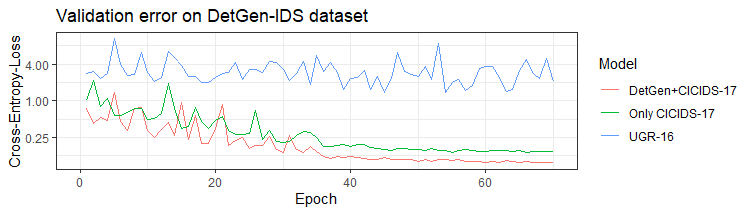
\includegraphics[width=0.99\textwidth]{images_SecureComm/ValLoss.png}
\caption{Validation errors of LSTM-model \cite{henryLSTM} on DetGen-IDS data.}\label{figM:ValLoss}
\end{figure}

In Fig. \ref{figM:ValLoss}, we compare the validation error of a recent LSTM-model for network intrusion detection by Clausen et al. \cite{henryLSTM} on the DetGen-IDS data to demonstrate that a model trained on the CICIDS-17 data is able to perform well without retraining. We distinguish models when trained exclusively on the CICIDS data (green), and when also trained on the probing data (red). 
% when trained exclusively on the CICIDS-17 dataset  and when also trained on the Probing dataset , as well as when trained on a third unrelated dataset for comparison (blue).
Even though the validation error is slightly higher when only trained on the CICIDS data, the difference is almost negligible compared to the error resulting from a model trained on a completely different dataset (UGR-16 \cite{macia2018ugr}, blue). This does not fully prove that every model is able to transfer observed structures between the two datasets, but it gives an indicator that they mirror characteristics.



\section{Conclusions}\label{SecM:Conclusion}

In this chapter, we described and examined a tool for generating traffic with controllable and extensively labelled traffic microstructures with the purpose of probing machine-learning-based traffic models. For this, we demonstrated the impact that probing with carefully crafted traffic microstructures can have for improving a model with a state-of-the-art LSTM-traffic-classifier with a detection rate that improved by more than 3\% after understanding how the model processes excessive network congestion. 

To verify DetGen's ability to control and monitor traffic microstructures, we performed experiments in which we quantified the experimental determinism of DetGen and compared it to traditional VM-based capture setups. Our similarity metrics indicate that traffic generated by DetGen is on average 10 times, and for connection sequences up to 30 times more consistent.

Alongside this work, we are releasing DetGen-IDS, a substantial dataset suitable for probing models trained on the CICIDS-17 dataset. This data should make it easier for researchers to understand where their model fails and what traffic characteristics are responsible to subsequently improve their design accordingly.

DetGen and the corresponding dataset are openly accessible for researchers on GitHub.


%By using HTTP-traffic with congestion settings, we were quickly able to identify the inability of an LSTM-based classifier to handle traffic with significant retransmission rates, which enabled us to improve the model accordingly and increase detection performance by more than $2\%$. Similarly, the examination of projection consistency of a subspace-clustering method using traffic with artificially similar characteristics revealed an overly high sensitivity to flow interarrival times, while cluster-coherence could be increased significantly by identifying half-open connections that were dropped because of network failure as the source of overly dispersed traffic projections. 

%These results have encouraged us to perform more deep-going probing of data-driven network intrusion detection models. We believe that in combination with strong NID-dataset, extensive model validation and corresponding development with targeted traffic samples might hold the key to reduce false positives of detection models to an acceptable rate, as well as help models replicate detection rates in practical settings.

\subsubsection*{Difficulties and limitations:}
%DetGen is building network traffic datasets from a small-scale level up by coalescing traffic from different fine-grained activities together. 
While the control of traffic microstructures helps to understand packet- or connection-level models, it does not replicate realistic network-wide temporal structures. Other datasets such as UGR-16 \cite{macia2018ugr} or LANL-15 \cite{turcotte17} are currently better suited to examine models of large-scale traffic structures.

While controlling traffic shaping factors artificially helps at identifying the limits and weak points of a model, it can exaggerate some characteristics in unrealistic ways and thus alter the actual detection performance of a model. 

The artificial randomisation of traffic shaping factors can currently not completely generate real-world traffic diversity. This problem is however more pronounced in commonly used synthetic datasets such as CICIDS-17, where for example most FTP-transfers consist of a client downloading the same text file.

Discussions about the implications of the model correction proposed in Section \ref{SecM:Motivation} are above the scope of this chapter, and there likely exist more complex and suitable solutions.

\subsubsection*{Future work:}
%These steps can also be applied for other synthetic datasets such as UNSW-NB15 that have sufficient information available in their documentation or the \texttt{pcap}-capture. Since DetGen already covered ALPs that are responsible for $98\%$  of connections in the CICIDS-17 data, it was most straightforward for us to generate probing data for the CICIDS-17 data.

%\subsubsection*{Import of activity timeline}

%The modelling and generation of computer network activity has been investigated extensively \textcolor{red}{(citations?)}, and tools to automatically generate realistic network activity streams 

%we do not wish to \textcolor{red}{address} this topic here . Instead, our framework imports existing time-series of \textcolor{red}{host flow activity} to generate the corresponding communication. \textcolor{red}{give more info on flow generation tools} 

%We transform existing network flow series into an activity timeline by \textcolor{red}{expand this}. We end up with an activity timeline that contains a set of timestamps along with the corresponding scenario and the source and destination host. 

%We paid meticulous attention to enable control over as many traffic impact factors as possible. However, 
DetGen is currently only offering insufficient control over underlying \textbf{application-layer implementations} such as TLS 1.3 vs 1.2. In theory, it should be unproblematic to provide containers with different implementations, and we are currently investigating how to compile containers in a suitable manner.

We are currently investigating how to better simulate causality in connection spawning and other \textbf{medium-term temporal dependencies}, such as by importing externally generated activity timelines from tools such as Doppelganger \cite{lin2019generating}. 

A project we are currently working on is to embed traffic scenarios into a larger and more complex \textbf{network topology} using MiniNet \cite{lantz2010network}.


%Working with Docker containers can sometimes complicate the implementation of individual scenarios compared to working with VMs. Although several applications are officially maintained Docker containers that are free from major errors, many do not. For instance, in the \textit{BitTorrent} scenario, most common command line tools, such as \texttt{mktorrent}, \texttt{ctorrent} and \texttt{buildtorrent}, failed to actually produce functioning torrent files from within a container due to Docker's union filesystem. Furthermore, due to the unique way in which we are using these software packages, unusual configuration settings are sometimes needed. %As such, many 

%Lastly, capturing \texttt{.pcap}-files from each container can quickly exceed available disc space when generating traffic at scale. Depending on specific research requirements, it is advisable to add filtering or feature extraction commands to the scenario execution scripts to enable traffic pre-processing in real-time.



%\subsection{Acknowledgement}
%We are grateful for our ongoing collaboration with our industry partners on this topic area, who provided both ongoing support and guidance to this work. Discussions with them have helped reinforce the need for a better evaluation and understanding of the possibilities that new intelligent tools can provide.

%Full funding sources after currently blinded.

